\chapter{Fading}
\label{ch:fading}

This chapter measures the problem. It asks how often an explanation names the entity that is really in the
passage, how often it names a wrong one, and how both change as the model reads on past the entity. All
results are on natural text.

\section{Fade Curve}

Start with what the activation holds. Table~\ref{tab:fade} shows how well the entity can be read from the
layer-20 activation at each distance, on all 1{,}800 test passages. At the entity's own token the probe is
right 99.9\% of the time. One token later it is right 59\% of the time, and by 16 tokens it is down to 31\%,
still three times chance.

\begin{table}[t]
\centering
\small
\begin{tabular}{@{}cll@{}}
\toprule
\shortstack[l]{Tokens after\\entity} & \shortstack[l]{Concept-vector\\readout} & Trained probe \\
\midrule
0 & 49.1 {\scriptsize[42.1, 56.2]} & 99.9 {\scriptsize[99.7, 100.0]} \\
1 & 30.2 {\scriptsize[25.1, 35.5]} & 59.2 {\scriptsize[55.3, 63.0]} \\
2 & 27.2 {\scriptsize[22.7, 31.8]} & 46.1 {\scriptsize[41.7, 50.6]} \\
4 & 25.8 {\scriptsize[21.3, 30.6]} & 39.6 {\scriptsize[35.4, 43.8]} \\
8 & 22.8 {\scriptsize[18.5, 27.4]} & 36.2 {\scriptsize[31.7, 40.8]} \\
16 & 22.4 {\scriptsize[18.7, 26.5]} & 31.2 {\scriptsize[26.9, 35.9]} \\
\bottomrule
\end{tabular}

\caption[Reading the entity from the activation]{Reading the entity from the activation: top-1 accuracy (\%)
among the ten entities of the same type, with 95\% intervals. Natural text, 1{,}800 test passages; chance is
10\%. The concept-vector readout needs no training data and is discussed in Chapter~\ref{ch:agreement}.}
\label{tab:fade}
\end{table}

Part of this drop is simply true of the model. A transformer does not need to carry the entity forward at
every position, because attention can look back at the token where it was read. An honest explanation of a
later activation should therefore mention the entity less often.

The question is whether the explanation fades at the same rate. Figure~\ref{fig:fade} and
Table~\ref{tab:names} put the verbalizer next to the probe on the same 540 passages.

\begin{figure}[t]
\centering
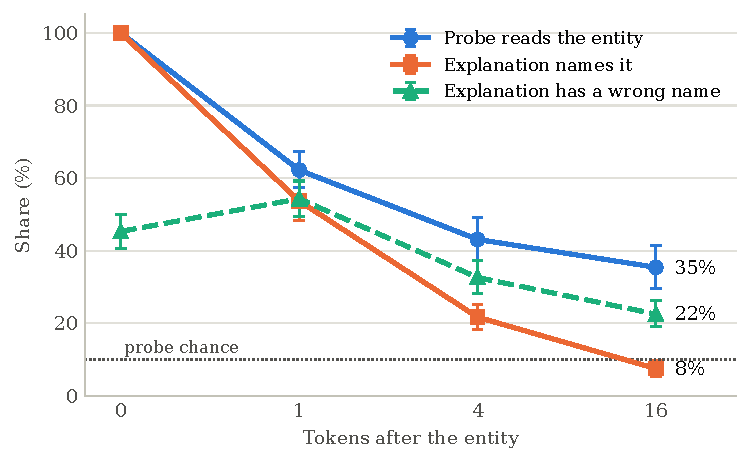
\includegraphics[width=0.78\linewidth]{fade}
\caption[The specific fades faster from the explanation than from the activation]{The specific fades faster
from the explanation than from the activation. Natural text, 540 held-out passages, four explanations per
activation; bars are 95\% intervals over entities. The dotted line is the probe's chance level; it does not
apply to the explanations, which are free text.}
\label{fig:fade}
\end{figure}

\begin{table}[t]
\centering
\footnotesize
\setlength{\tabcolsep}{4pt}
\begin{tabular}{@{}cllllc@{}}
\toprule
\shortstack[l]{Tokens after\\entity} & Probe reads it & \shortstack[l]{Names the true\\entity} & \shortstack[l]{At least one\\wrong name} & \shortstack[l]{Only wrong\\names} & \shortstack[l]{Wrong names\\per\\explanation} \\
\midrule
0 & 100.0 {\scriptsize[100.0, 100.0]} & 100.0 {\scriptsize[99.9, 100.0]} & 45.3 {\scriptsize[40.7, 49.9]} & 0.0 {\scriptsize[0.0, 0.1]} & 0.72 \\
1 & 62.2 {\scriptsize[57.4, 67.2]} & 53.7 {\scriptsize[48.3, 59.2]} & 54.3 {\scriptsize[49.5, 59.2]} & 25.1 {\scriptsize[21.5, 28.9]} & 1.10 \\
4 & 43.1 {\scriptsize[37.4, 49.1]} & 21.7 {\scriptsize[18.2, 25.2]} & 32.6 {\scriptsize[28.1, 37.3]} & 23.5 {\scriptsize[19.8, 27.2]} & 0.52 \\
16 & 35.4 {\scriptsize[29.6, 41.5]} & 7.5 {\scriptsize[5.4, 9.8]} & 22.5 {\scriptsize[19.0, 26.3]} & 20.0 {\scriptsize[16.7, 23.6]} & 0.33 \\
\bottomrule
\end{tabular}

\caption[What the explanations name]{What the explanations name, in \% of explanations with 95\% intervals.
Natural text, 540 passages, 8{,}640 explanations. ``Only wrong names'' means the explanation names a wrong
same-type entity and not the true one. The first column is the probe's accuracy on the same passages.}
\label{tab:names}
\end{table}

At distance~0 the two agree: the explanation names the entity in all but one of 2{,}160 cases. After that
they part. At 4 tokens the probe reads the entity 43\% of the time and the explanation names it 22\% of the
time. At 16 tokens it is 35\% against 7.5\%. The verbalizer is leaving on the table between half and four
fifths of what a simple linear reader can still get.

This comparison is somewhat unfair to the verbalizer: the probe must answer every time, while the verbalizer
can stay silent. Table~\ref{tab:fair} corrects for that by scoring the probe only on its most confident
passages, as many as the verbalizer chose to name something in.

\begin{table}[t]
\centering
\small
\begin{tabular}{@{}ccll@{}}
\toprule
\shortstack[l]{Tokens after\\entity} & \shortstack[l]{Names any\\same-type\\entity} & \shortstack[l]{Verbalizer\\precision} & \shortstack[l]{Probe, equally\\selective} \\
\midrule
0 & 100.0\% & 100.0 {\scriptsize[99.9, 100.0]} & 100.0 {\scriptsize[100.0, 100.0]} \\
1 & 78.9\% & 68.1 {\scriptsize[63.1, 72.9]} & 69.2 {\scriptsize[64.1, 74.0]} \\
4 & 45.2\% & 48.1 {\scriptsize[41.7, 54.4]} & 50.8 {\scriptsize[41.5, 60.9]} \\
16 & 27.5\% & 27.2 {\scriptsize[20.4, 34.2]} & 52.7 {\scriptsize[42.4, 63.4]} \\
\bottomrule
\end{tabular}

\caption[The verbalizer against an equally selective probe]{The verbalizer against an equally selective
probe (\%, 95\% intervals; natural text). Precision is the share of naming explanations that name the true
entity. The probe is scored on its most confident passages, as many as the verbalizer chose to name.}
\label{tab:fair}
\end{table}

At 1 and 4 tokens, when the verbalizer names something it is about as accurate as the equally selective
probe: 68\% against 69\%, and 48\% against 51\%. Its lower true-name rate there comes from speaking less
often, which is defensible. At 16
tokens the two separate: the verbalizer's precision is 27\%, the probe's is 53\%. Far from the entity, when
the verbalizer names something of the right type, it names the wrong thing three times out of four.

\section{Wrong Names}
\label{sec:wrongnames}

The orange line in Figure~\ref{fig:fade} falling would be harmless on its own. What makes it a problem is
the green line. At every distance a large share of explanations contain at least one wrong name of the
entity's type: 45\% at the entity's token, 54\% one token later, and still 22\% at 16 tokens
(Table~\ref{tab:names}).

Two things stand out. First, wrong names are common even at distance~0, where the true name is always
present. There the explanation typically names the right entity and then adds others around it. In one
example about a recording of Beethoven's Spring sonata, the explanation correctly quotes ``and Beethoven''
but also invents ``Mozart's complete piano sonatas'' as the preceding item. Second, as the true name
disappears the wrong names do not disappear with it. By 16 tokens, an explanation that names any entity of
the type is far more likely to be naming only a wrong one (20\% of all explanations) than the true one
(7.5\%).

The wrong names are not drawn from my list of 60. At 4 tokens, 77\% of them are same-type entities outside
the list, and at 16 tokens 82\%. The most common are everyday members of the type: guitar, dog, piano and
lion at 4 tokens; Toronto, piano, guitar and Italy at 16. They look like what one would guess knowing only
the type. Here is a typical case, four tokens after \emph{Moscow}:

\begin{sample}{Passage (read to four tokens past \emph{Moscow})}
\ldots At nine, Forough was the youngest ever to be admitted to the Royal Conservatory of Music, Brussels as
a pupil of Arthur Grumiaux. Later studies were with David Oistrakh at the \true{Moscow} Conservatory. \ldots
\end{sample}

\begin{sample}{Explanation}
Wikipedia biographical article format with English language entries on Ukrainian tenor Vladimir Ashkenazy,
detailing career and musical achievements. The sentence structure ``Ashkenazy studied music in
\wrong{Paris} beginning in 1952, and won international competitions \ldots''
\end{sample}

The gist is intact: a biography of a classical musician with Soviet connections, studying at a conservatory
in a capital city. The city is wrong, and so is the musician.

\section{Name Position}

Each explanation describes the context and then predicts what comes next. A wrong name in the prediction
(``expecting \emph{Paris} or \emph{London}'') is a guess labelled as a guess. A wrong name in the description
of the context is a false statement about what the model read. Table~\ref{tab:position} separates the two,
cutting each explanation at the phrase that introduces its predicted continuation.

\begin{table}[t]
\centering
\small
\setlength{\tabcolsep}{5pt}
\begin{tabular}{@{}cllll@{}}
\toprule
\shortstack[l]{Tokens after\\entity} & \shortstack[l]{True name,\\context} & \shortstack[l]{True name,\\continuation} & \shortstack[l]{Wrong name,\\context} & \shortstack[l]{Wrong name,\\continuation} \\
\midrule
0 & 100.0 {\scriptsize[99.9, 100.0]} & 11.1 {\scriptsize[8.1, 14.6]} & 35.8 {\scriptsize[32.2, 39.4]} & 17.9 {\scriptsize[14.5, 21.5]} \\
1 & 53.1 {\scriptsize[47.5, 58.6]} & 7.8 {\scriptsize[5.9, 9.8]} & 51.7 {\scriptsize[47.0, 56.4]} & 15.3 {\scriptsize[12.5, 18.2]} \\
4 & 20.5 {\scriptsize[17.0, 24.0]} & 3.2 {\scriptsize[2.0, 4.5]} & 30.2 {\scriptsize[26.0, 34.6]} & 7.7 {\scriptsize[6.0, 9.5]} \\
16 & 6.7 {\scriptsize[4.7, 8.8]} & 1.4 {\scriptsize[0.7, 2.1]} & 20.8 {\scriptsize[17.4, 24.4]} & 4.8 {\scriptsize[3.5, 6.2]} \\
\bottomrule
\end{tabular}

\caption[Where names sit in the explanation]{Where names sit in the explanation: \% of explanations with a
true or wrong name in the part that describes the context, and in the part that predicts the continuation.
Natural text; 95\% intervals.}
\label{tab:position}
\end{table}

Most wrong names are in the description, not the prediction. One token after the entity, 52\% of
explanations have a wrong name in the context part and 15\% have one in the continuation part; in raw
counts, 1{,}993 wrong names against 495. The ratio is between two and five to one at every distance. The problem is
therefore not that the verbalizer hedges with a list of candidates for the next word. It states, as a
description of the text, things that are not in the text.

In short, the specific fades faster from the explanation than from the activation, and what takes its place
is a plausible wrong name stated as fact.
